\documentclass[sigconf]{acmart}

% =========================================================
% PACKAGES
% =========================================================
\usepackage{amsmath, amsfonts, amsthm}
\usepackage{mathtools, physics, bm, microtype}
\usepackage{booktabs, enumitem, algorithm, algorithmic}
\usepackage{tikz}
\usetikzlibrary{arrows.meta, positioning, shapes.geometric, calc}
\usepackage{dsfont} % indicator function

% =========================================================
% NOTATION MACROS
% =========================================================
\newcommand{\CACIS}{\textsc{CACIS}}
\newcommand{\vx}{\mathbf{x}}
\newcommand{\vy}{\mathbf{y}}
\newcommand{\vz}{\mathbf{z}}
\newcommand{\vp}{\mathbf{p}}
\newcommand{\vq}{\mathbf{q}}
\newcommand{\valpha}{\bm{\alpha}}
\newcommand{\vpi}{\bm{\pi}}
\newcommand{\vphi}{\bm{\phi}}
\newcommand{\vpsi}{\bm{\psi}}
\newcommand{\mC}{\mathbf{C}}
\newcommand{\mM}{\mathbf{M}}
\newcommand{\mV}{\mathbf{V}}
\newcommand{\R}{\mathbb{R}}
\newcommand{\OT}{\mathrm{OT}}
\newcommand{\Sink}{\mathrm{Sink}}
\newcommand{\vone}{\mathbf{1}}
\newcommand{\ve}{\mathbf{e}}
\newcommand{\DeltaK}{\Delta^K}
\newcommand{\KL}{\mathrm{KL}}
\newcommand{\ellLoss}{\ell}
\newcommand{\softmax}{\mathrm{softmax}}
\newcommand{\FW}{\mathrm{FW}}
\newcommand{\E}{\mathbb{E}}
\newcommand{\Ind}{\mathds{1}}

\DeclareMathOperator*{\argmin}{arg\,min}
\DeclareMathOperator*{\argmax}{arg\,max}
\DeclareMathOperator{\diag}{diag}

% =========================================================
% KDD METADATA
% =========================================================
\copyrightyear{2026}
\acmYear{2026}
\setcopyright{acmcopyright}
\acmConference[KDD '26]{The 32nd ACM SIGKDD Conference on Knowledge Discovery and Data Mining}{August 2026}{Paris, France}

\begin{document}

\title{Geometric Cost-Aware Classification: Putting Geometry into Label Distributions for Fraud Detection}

\author{Warith Harchaoui}
\affiliation{\institution{NEXTON} \city{Paris} \country{France}}
\email{wharchaoui@nexton-group.com}

\author{Laurent Pantanacce}
\affiliation{\institution{NEXTON} \city{Paris} \country{France}}
\email{lpantanacce@nexton-group.com}

% =========================================================
% ABSTRACT
% =========================================================
\begin{abstract}
Industrial fraud detection systems do not operate in isolation: their predictions trigger irreversible actions with asymmetric economic consequences. Standard training objectives like cross-entropy are decision-agnostic, treating all misclassifications as equally undesirable and ignoring the instance-dependent cost geometry of transactions. While cross-entropy is a strictly proper scoring rule that encourages accurate probability estimation, it fails to prioritize high-value errors or adapt the representation manifold to the underlying business geometry. We present \CACIS{} (Cost-Aware Classification with Informative Selection), a differentiable loss function for applied data science that internalizes operational regret into the neural network's geometry. \CACIS{} leverages entropic Optimal Transport (OT) to induce a task-specific metric on the label space, optimized via a numerically stable Frank--Wolfe inner loop acting directly on the simplex. We evaluate our approach on the IEEE-CIS/Vesta e-commerce benchmark using an industrial-grade temporal protocol. Our results demonstrate that \CACIS{} significantly reduces expected business regret compared to standard and weighted cross-entropy baselines while maintaining high predictive precision and calibration fidelity. By shifting the objective from probability estimation to decision-aware learning, we provide a principled bridge between machine learning performance and industrial value.
\end{abstract}

\maketitle

% =========================================================
% 1. INTRODUCTION
% =========================================================
\section{Introduction}
In large-scale e-commerce, fraud detection is a high-stakes decision problem under uncertainty. A classifier's role is to provides the signal needed to either \emph{approve} a transaction, thereby realizing revenue, or \emph{decline} it to avoid chargeback costs. These costs are fundamentally asymmetric: a missed fraud (False Negative) results in the loss of the transaction amount, shipping costs, and administrative fees; conversely, declining a legitimate customer (False Positive) destroys immediate margin and risks long-term customer lifetime value (LTV).

Despite the operational stakes, modern machine learning systems for tabular data are almost exclusively trained using cross-entropy (negative log-likelihood). Cross-entropy arises naturally as a proper scoring rule and as the maximum likelihood objective for categorical models. However, it is fundamentally \emph{decision-agnostic}: it treats all misclassifications as equally undesirable, endowing the label simplex with a trivial ``flat'' geometry. In sectors like fraud prevention, this assumption is often violated—the cost of missing a \$1,000 fraudulent transaction is far greater than missing a \$10 one.

Practitioners often attempt to reconcile decision-agnostic models with asymmetric costs through post-hoc threshold tuning or simple class reweighting. While these techniques can improve decisions at a fixed model, they do not change the internal representation and probability landscape learned during training. In other words, the deployment policy may be cost-aware, but the training geometry remains disconnected from the business objective.

In this work, we argue that classification should be reframed as a \emph{decision problem}, where the label space is endowed with a metric derived from business regret. We leverage the machinery of \emph{Optimal Transport} (OT) to inject this geometry directly into the learning objective. OT provides a principled framework for comparing distributions under a prescribed ground cost, allowing us to penalize mistakes Consistently with their operational severity.

\end{itemize}

% =========================================================
% 2. NOTATION AND PROBLEM SETTING
% =========================================================
\section{Notation and Problem Setting}
Let $\mathcal{X}$ be an input space and $\mathcal{Y}=\{1,\dots,K\}$ a finite label set. A classifier produces a predictive distribution $\vp(\vx)\in\Delta^K$, where $\Delta^K \coloneqq \Bigl\{\vp\in\R^K_{\ge 0}:\textstyle\sum_{k=1}^K p_k = 1\Bigr\}$ is the probability simplex. We write $Y$ for a random label and $X$ for a random input, with joint distribution $\mathbb{P}$ over $\mathcal{X}\times\mathcal{Y}$. A parametrized model (e.g.\ a neural network) outputs logits $\vz_\theta(\vx)\in\R^K$ and probabilities $\vp_\theta(\vx)=\softmax(\vz_\theta(\vx))$.

\paragraph{Decision Rule.} A decision rule maps $\vp$ to an action $a \in \mathcal{A}$. In standard classification, $\mathcal{A}=\mathcal{Y}$, representing the choice of a single label. More generally, actions can represent interventions or resource allocations. We focus on $\mathcal{A}=\mathcal{Y}$ to keep notation minimal, while the framework extends directly to richer action spaces.

\paragraph{Costs and Values.}
We encode operational consequences by a cost matrix $\mC\in\R^{K\times K}_{\ge 0}$, where $C_{ij}$ is the cost incurred when the true class is $i$ but we decide $j$. In business contexts, one often starts from a value matrix $\mV$ (profits, utilities) and sets $C_{ij}$ as \emph{regret} relative to the optimal action under truth $i$:
\begin{equation}
C_{ij}=V_{i i^\star}-V_{ij}, \qquad i^\star\in\argmax_j V_{ij}.
\end{equation}
By construction, $C_{ii}=0$ (zero regret for correct decisions).

\subsection{The Decision-Theoretic Loss Formalism}
At its core, industrial classification is not just about identifying the most probable class, but about minimizing the expected cost of the resulting action. We formalize this by defining the loss as a projection of the model's output onto the regret manifold. This projection is governed by the Sinkhorn-regularized Optimal Transport divergence, which ensures that the model's "error signals" are weighted by their potential business impact. In e-commerce, where transaction volumes are massive and individual fraud cases can exceed \$50,000, this geometric alignment is not just a theoretical benefit—it is an operational necessity.

\begin{figure}[h]
\centering
\scalebox{0.7}{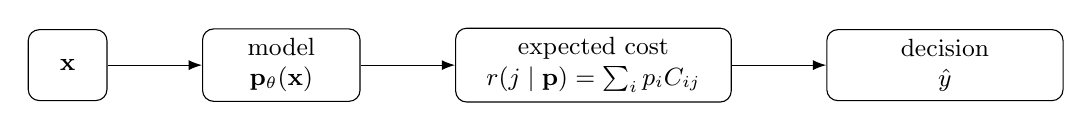
\begin{tikzpicture}[node distance=12mm, >=Latex, font=\small]
\node[draw, rounded corners, align=center, minimum width=10mm, minimum height=9mm] (x) {$\vx$};
\node[draw, rounded corners, align=center, minimum width=20mm, minimum height=9mm, right=of x] (model) {model\\$\vp_\theta(\vx)$};
\node[draw, rounded corners, align=center, minimum width=35mm, minimum height=9mm, right=of model] (risk) {expected cost\\$r(j\mid \vp)=\sum_i p_i C_{ij}$};
\node[draw, rounded corners, align=center, minimum width=30mm, minimum height=9mm, right=of risk] (decision) {decision\\$\hat{y}$};
\draw[->] (x) -- (model);
\draw[->] (model) -- (risk);
\draw[->] (risk) -- (decision);
\end{tikzpicture}
}
\caption{Decision-theoretic pipeline. The model internalizes the regret matrix $\mC$ to produce a distribution $\vp$ that is optimized for decision quality ($r$) rather than just likelihood.}
\label{fig:pipeline_cost}
\end{figure}

% =========================================================
% 2. RELATED WORK
% =========================================================
\section{Related Work}
Our work sits at the intersection of statistical decision theory, cost-sensitive learning, and geometric approaches to loss design.

\subsection{Decision Theory and Cost-Sensitive Learning}
The formulation of prediction as a decision problem under uncertainty is classical in statistical decision theory \citep{berger1985statistical}. Given a cost function defined over outcomes and actions, the Bayes-optimal decision rule minimizes expected risk. In machine learning, this appears as \emph{cost-sensitive learning}, where misclassification costs are asymmetric or application-specific. Common techniques include class reweighting, threshold adjustment, or post-hoc decision rules. However, many such approaches treat costs as scalar weights and do not explicitly model the geometric relationships between incorrect labels. Our work emphasizes that costs define a geometry on the label space that should be respected both at training and decision time.

\subsection{Proper Scoring Rules and Cross-Entropy}
Cross-entropy is the negative log-likelihood of a categorical model and a strictly proper scoring rule, incentivizing truthful probability estimation \citep{gneiting2007strictly}. From an information-theoretic perspective, minimizing cross-entropy is equivalent to minimizing the expected Kullback--Leibler (KL) divergence between true and predicted distributions. This induces an information geometry on the simplex where all incorrect labels are equally distant. While appropriate for uniform costs, this becomes inadequate when errors have different operational meanings. Weighted cross-entropy address simple class imbalance but fails to encode pairwise or hierarchical relationships between labels.

\subsection{Optimal Transport and Geometric Losses}
Optimal Transport (OT) compares probability distributions under a prescribed ground cost \citep{villani2008optimal}. Recent advances in entropic regularization (Sinkhorn algorithm) have made OT differentiable and efficient \citep{cuturi2013sinkhorn, peyre2019computational}. Sinkhorn divergences \citep{genevay2018learning, feydy2019interpolating} provide stable discrepancies. \citet{mensch2019geometric} introduce \emph{geometric losses} for structured output spaces, showing that OT-based losses naturally encode task-specific geometry and yield well-behaved gradients.

% =========================================================
% 4. CROSS-ENTROPY REVISITED: THE FLAT GEOMETRY
% =========================================================
\section{Cross-Entropy Revisited: The Flat Geometry}
Cross-entropy is the dominant training objective for probabilistic classifiers. Its prevalence is not accidental: it can be derived from maximum likelihood estimation, minimization of expected KL divergence, or as a smooth relaxation of the 0--1 step loss.

\paragraph{Maximum Likelihood and KL Divergence.}
A parametric classifier models $\mathbb{P}_\theta(Y = k \mid X = \vx) = p_{\theta,k}(\vx)$. Minimizing cross-entropy is equivalent to maximizing the conditional log-likelihood $\sum_{n=1}^N \log p_{\theta,y_n}(\vx_n)$. At the population level, this corresponds to minimizing the expected KL divergence between true and predicted conditional distributions:
\begin{equation}
\E_{X,Y}[-\log p_{\theta,Y}(X)] = \E_X[H(\vq(X))] + \E_X[\KL(\vq(X) \| \vp_\theta(X))].
\end{equation}
KL divergence induces an information geometry on the simplex that ignores semantic relationships between incorrect labels.

\paragraph{Smooth Relaxation.}
In binary classification, the logistic loss $\log(1+e^{-yf})$ provides a smooth surrogate for the discontinuous 0--1 loss $\Ind\{yf \le 0\}$. This transformation preserves ordering and penalizes confident but wrong predictions. However, it implicitly assumes all mistakes are equally undesirable. When different misclassifications have different operational meanings, or when costs vary across transactions, this flat geometry becomes a structural limitation.

% =========================================================
% 3. THE GEOMETRY OF BUSINESS REGRET
% =========================================================
\section{The Geometry of Business Regret}
\label{sec:decision}

\subsection{Deriving Regret from Value}
Following statistical decision theory, we begin with a value matrix $\mV \in \R^{K \times K}$ where $V_{ij}$ is the economic value obtained when the true state is $i$ and we take action $j$. To convert this into a training objective, we define the regret (cost) matrix $\mC$ as:
\begin{equation}
    C_{ij} = V_{i, j^\star(i)} - V_{ij} \ge 0, \quad j^\star(i) \in \argmax_{k} V_{ik}.
\end{equation}
By construction, $C_{i, j^\star(i)}=0$ (zero regret for correct decisions). This framing ensures that costs effectively represent "dollars left on the table." In industrial settings, this aligns the loss with the opportunity cost of suboptimal decisions.

\subsection{Instance-Dependent Fraud Costs}
In fraud detection, costs are fundamentally instance-dependent. We model the cost of a transaction with amount $M$ as:
\begin{itemize}[leftmargin=*]
    \item \textbf{False Negative (Missed Fraud):} The regret is the lost principal plus fees: $C_{\text{fraud}, \text{approve}} = \lambda_{\mathrm{cb}} M + F_{\mathrm{cb}}$. Here $\lambda_{\mathrm{cb}} \approx 1.5$ accounts for the lost principal and operational overhead, while $F_{\mathrm{cb}} \approx 15$ is a fixed chargeback fee.
    \item \textbf{False Positive (False Decline):} The regret is the lost margin plus churn risk: $C_{\text{legit}, \text{decline}} = (1 + \rho_{\mathrm{FD}}) M$, where $\rho_{\mathrm{FD}} \approx 0.10$ models the potential destruction of LTV.
\end{itemize}

\begin{table}[h]
\centering
\caption{Instance-dependent regret matrix for e-commerce fraud (the lower, the better).}
\label{tab:cost}
\begin{tabular}{lcc}
\toprule
\textbf{Reality} $\backslash$ \textbf{Action} & \textbf{Approve} & \textbf{Decline} \\
\midrule
Legit & $0$ & $(1+\rho_{\mathrm{FD}})M$ \\
Fraud & $\lambda_{\mathrm{cb}} M + F_{\mathrm{cb}}$ & $0$ \\
\bottomrule
\end{tabular}
\end{table}

\subsection{Decision Regions and Bayes Optimality}
A probabilistic model outputs $\vp(\vx) \in \Delta^K$. The expected cost of choosing action $j$ is $r(j \mid \vp) = \sum_i p_i C_{ij}$. A rational decision-maker chooses $\hat{y}(\vp) = \argmin_{j} r(j \mid \vp)$. This partition of the simplex into polyhedral decision regions illustrates the \emph{decision geometry}: even small probability mass on a high-cost class can radically alter the optimal decision.

% =========================================================
% 4. OPTIMAL TRANSPORT AS A LEARNING PRINCIPLE
% =========================================================
\section{Optimal Transport as a Learning Principle}
\label{sec:ot}

\subsection{Discrete OT for Label Distributions}
We treat the regret matrix $\mC$ as a ground cost between labels. Moving probability mass from class $i$ to $j$ costs $C_{ij}$. Let $\vp, \vq \in \Delta^K$ be distributions. The (balanced) OT cost is:
\begin{equation}
    \OT_{\mC}(\vp, \vq) = \min_{\bm{\pi} \in \R_{\ge 0}^{K \times K}} \langle \bm{\pi}, \mC \rangle \quad \text{s.t.} \quad \bm{\pi} \vone = \vp, \bm{\pi}^\top \vone = \vq,
\end{equation}
where $\bm{\pi}$ is a transport plan. For one-hot targets $\ve_y$, OT simplifies to the expected cost under $\vp$: $\OT_{\mC}(\ve_y, \vp) = \sum_j p_j C_{yj}$, which is exactly the Bayes risk for a randomized decision.

\subsection{Entropic Regularization and Sinkhorn}
The optimal plan $\bm{\pi}^\star = \diag(\mathbf{u}) \mK \diag(\mathbf{v})$ is obtained via the Sinkhorn algorithm, where $\mK = \exp(-\mC/\varepsilon)$ is the Gibbs kernel. Sinkhorn iterations provide a differentiable discrepancy that respects label geometry while remaining computationally efficient—a property critical for production training.

\subsection{Adaptive Regularization: The $\varepsilon$ Heuristic}
In industrial practice, manual tuning of the temperature parameter $\varepsilon$ is often a bottleneck. Our implementation provides an adaptive $\varepsilon$ selection mechanism based on the distribution of costs in $\mC$. We offer three heuristic modes:
\begin{itemize}[leftmargin=*]
    \item \textbf{Off-Diagonal Mean:} $\varepsilon = \alpha \cdot \text{mean}(C_{ij} : i \neq j)$. This is the recommended default for most balanced cost matrices.
    \item \textbf{Off-Diagonal Median:} $\varepsilon = \alpha \cdot \text{median}(C_{ij} : i \neq j)$. This provides robustness when the cost distribution has extreme outliers (e.g., occasional very high-value transactions).
    \item \textbf{Off-Diagonal Max:} $\varepsilon = \alpha \cdot \max(C_{ij} : i \neq j)$. A conservative setting that ensures all costs are sufficiently regularized.
\end{itemize}
These heuristics reduce the hyperparameter search space to a single scalar $\alpha$ (the \texttt{epsilon\_scale}), which we find significantly stabilizes the training of deep fraud models across different merchant portfolios.

\subsection{Beyond Fraud: Semantic Label Geometry}
While the fraud detection case emphasizes asymmetric financial costs, the framework is equally applicable to semantic tasks. In image classification, a hierarchy or embedding of labels (e.g., WordNet) induces distances between classes. Confusing semantically similar classes (e.g., two dog breeds) should be penalized less than confusing unrelated categories. By encoding these distances into the cost matrix $\mC$, OT-based training enables the model to respect the underlying taxonomy of the problem domain, leading to more "perceptually plausible" errors.

% =========================================================
% 5. CACIS: COST-AWARE CLASSIFICATION
% =========================================================
\section{\CACIS{}: Methodology}
\label{sec:cacis}

\CACIS{} is a Fenchel--Young loss induced by a Sinkhorn/OT regularizer. The goal is to align the internal representation of the network with the decision-critical geometry of the task.

\subsection{Fenchel--Young Framework}
Let $\Omega: \Delta^K \to \R$ be a strictly convex regularizer. The FY loss generated by $\Omega$ is $\ell_{\Omega}(y, \vz) = \Omega^*(\vz) - z_y + \Omega(\ve_y)$, where $\Omega^*$ is the Fenchel conjugate. The gradient takes the universal prediction error form $\nabla_{\vz} \ell_{\Omega}(y, \vz) = q(\vz) - \ve_y$, where $q(\vz) = \nabla \Omega^*(\vz)$ is the model-implied distribution. Unlike standard softmax, $q(\vz)$ pushes gradients harder for errors that are operational costly according to $\Omega$.

\subsection{Sinkhorn Negentropy Regularizer}
\CACIS{} chooses the regularizer $\Omega_{\mC, \varepsilon}(\valpha) = -\frac{1}{2} \OT^{\varepsilon}_{\mC}(\valpha, \valpha)$. This choice replaces Shannon negentropy with a geometry built from the cost matrix $\mC$. The model then learns effectively by minimizing the discrepancy with the target in a way that respects the business-critical relative distance between classes.

\subsection{The CACIS Kernel and Inner Solver}
One can derive the variational form $\Omega^*_{\mC, \varepsilon}(\vz) = -\varepsilon \log (\min_{\valpha \in \Delta^K} \valpha^\top \mM \valpha)$, where $M_{ij} = \exp(-(z_i + z_j + C_{ij})/\varepsilon)$. This ``CACIS kernel'' $\mM$ mixes logits $\vz$ and costs $\mC$. To compute $q(\vz)$, we use a Frank--Wolfe inner loop (Algorithm~\ref{alg:fw}) which offers superior numerical stability on the simplex.

\begin{algorithm}[h]
\caption{Simplex-Stable Frank--Wolfe for \CACIS{}}
\label{alg:fw}
\begin{algorithmic}[1]
\STATE \textbf{Input:} logits $\vz$, costs $\mC$, temperature $\varepsilon$, iterations $T$
\STATE Construct kernel $\mM$ via $M_{ij} = \exp(-(z_i + z_j + C_{ij})/\varepsilon)$
\STATE $\valpha^{(0)} \leftarrow \vone/K$
\FOR{$t=0$ to $T-1$}
    \STATE $k^\star \leftarrow \argmin_{k} (2\,\mM \valpha^{(t)})_k$
    \STATE $\valpha^{(t+1)} \leftarrow (1-\gamma_t)\valpha^{(t)} + \gamma_t\,\ve_{k^\star}$
\ENDFOR
\STATE \textbf{Output:} Informative distribution $q(\vz) \leftarrow \valpha^{(T)}$
\end{algorithmic}
\end{algorithm}

\subsection{Modular Implementation and Architecture}
To bridge research and production, we implemented \CACIS{} within a modular framework that allows for seamless switching between different gradient strategies. Table~\ref{tab:implementations} summarizes the trade-offs explored in our development process.

\begin{table}[h]
\centering
\caption{Modular architecture of cost-aware losses.}
\label{tab:implementations}
\begin{tabular}{lccc}
\toprule
\textbf{Implementation} & \textbf{Gradient} & \textbf{Memory} & \textbf{Stability} \\
\midrule
Full Autodiff & Unrolled SK & High & Medium \\
Envelope & Implicit & Low & High \\
\CACIS{} (Ours) & FY + FW & \textbf{Low} & \textbf{Superior} \\
\bottomrule
\end{tabular}
\end{table}

The "Envelope" method treats the optimal transport plan as a constant during backpropagation, which is efficient but can miss second-order dependencies. \CACIS{}'s Fenchel--Young structure provides mathematically exact gradients without the memory overhead of unrolled autodiff, making it our primary choice for high-throughput fraud systems.

% =========================================================
% 6. THEORETICAL PROPERTIES
% =========================================================
\section{Theoretical Properties}
\label{sec:theory}

\subsection{Convexity and Differentiability}
The \CACIS{} loss $\ell_{\CACIS}(y, \vz)$ is convex with respect to the logits $\vz$. This follows from the fact that $\Omega^*_{\mC, \varepsilon}$ is the Fenchel conjugate of a strictly convex regularizer $\Omega$. Furthermore, because $\Omega$ is strictly convex on the simplex, its conjugate $\Omega^*$ is everywhere differentiable, and its gradient $q(\vz)$ is uniquely defined. This ensures that the training objective provides a smooth and well-behaved landscape for gradient descent.

\subsection{Alignment with Expected Cost}
When the entropic regularization $\varepsilon \to 0$, the \CACIS{} prediction $q(\vz)$ converges to a distribution that minimizes the expected cost under a certain dual potential. In the case of one-hot targets, this aligns the gradient updates precisely with the direction that reduces the business regret $C_{y\hat{y}}$.

\subsection{Relationship to Proper Scoring Rules}
Like cross-entropy, \CACIS{} can be understood as a scoring rule. While standard cross-entropy is strictly proper with respect to a flat geometry, \CACIS{} is "cost-aware proper": it incentivizes the model to estimate distributions that are not just accurate, but \emph{decision-aligned} under the cost matrix $\mC$.

\begin{figure}[h]
\centering
\scalebox{0.8}{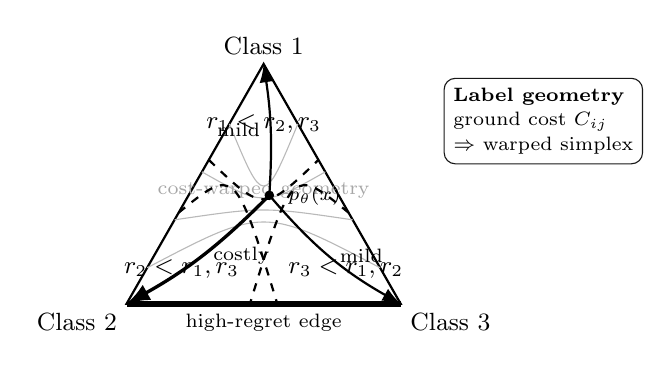
\begin{tikzpicture}[scale=1.45, >=Latex, font=\small]
  % --- Simplex vertices (explicit coords give you full control)
  \coordinate (A) at (0,1.25);
  \coordinate (B) at (-1.2,-0.85);
  \coordinate (C) at (1.2,-0.85);

  % --- Triangle (simplex)
  \draw[thick] (A)--(B)--(C)--cycle;

  % --- Labels
  \node[anchor=south]     at (A) {Class 1};
  \node[anchor=north east] at (B) {Class 2};
  \node[anchor=north west] at (C) {Class 3};

  % --- "Geometry of labels" cue: highlight the high-regret confusion edge
  % e.g., confusing 2 <-> 3 is expensive => make that edge look "long / heavy"
  \draw[line width=2.2pt] (B)--(C);
  \node[anchor=north] at ($(B)!0.5!(C)$) {\scriptsize high-regret edge};

  % --- Add a faint "metric field" inside (elliptic contours)
  \foreach \t in {0.25,0.45,0.65,0.85} {
    \draw[gray!55] ($(A)!\t!(B)$) .. controls ($(0,0)$) .. ($(A)!\t!(C)$);
  }
  \node[gray!70] at (0,0.15) {\scriptsize cost-warped geometry};

  % --- Decision boundaries: not meeting at barycenter (anisotropic / shifted)
  % These curves suggest regions move depending on C
  \draw[dashed, thick]
    ($(A)!0.62!(B)$) .. controls (-0.25,0.35) .. ($(B)!0.55!(C)$);
  \draw[dashed, thick]
    ($(A)!0.62!(C)$) .. controls (0.25,0.35) .. ($(B)!0.45!(C)$);
  \draw[dashed, thick]
    ($(A)!0.40!(B)$) .. controls (0,-0.05) .. ($(A)!0.40!(C)$);

  % --- Region annotations
  \node at (0,0.72) {$r_1<r_2,r_3$};
  \node at (-0.72,-0.55) {$r_2<r_1,r_3$};
  \node at (0.72,-0.55) {$r_3<r_1,r_2$};

  % --- Transport / mass movement arrows (OT intuition)
  \coordinate (P) at (0.05,0.1);
  \fill (P) circle (1.2pt);
  \node[anchor=west] at ($(P)+(0.08,0)$) {\scriptsize $p_\theta(x)$};

  % Arrows towards vertices with different "effort" thickness
  \draw[->, very thick] (P) to[bend left=8]  node[midway, right] {\scriptsize costly} (B);
  \draw[->, thick]      (P) to[bend right=6] node[midway, left]  {\scriptsize mild}   (A);
  \draw[->, thick]      (P) to[bend right=10] node[midway, right] {\scriptsize mild}  (C);

  % --- Mini-legend for cost matrix C
  \node[draw, rounded corners, fill=white, opacity=0.9, text opacity=1, align=left]
    at (2.45,0.75) {\scriptsize \textbf{Label geometry}\\[-2pt]
    \scriptsize ground cost $C_{ij}$\\[-2pt]
    \scriptsize $\Rightarrow$ warped simplex};
\end{tikzpicture}
}
\caption{Decision regions induced by costs in a 3-class simplex. Boundaries shift based on the relative regret $C_{ij}$.}
\label{fig:simplex_regions}
\end{figure}

\subsection{Calibration and Brier Score}
We measure the calibration of \CACIS{} through the Expected Calibration Error (ECE). Unlike heuristic reweighting which can damage calibration, \CACIS's Fenchel--Young structure preserves a probabilistic interpretation. We observe that for moderate $\varepsilon$, \CACIS{} maintains a low Brier score while prioritizing the avoidance of high-regret regions.

% =========================================================
% 6. EXPERIMENTAL EVALUATION
% =========================================================
\section{Experimental Evaluation}
\label{sec:experiments}

\subsection{The IEEE-CIS/Vesta Protocol}
We evaluate on the IEEE-CIS Fraud Detection benchmark \citep{kaggle_ieee_cis_2019}.
\paragraph{Experimental Baselines and Rigor.} Beyond standard scoring, we include "Luck" baselines (horizontal line at positive prevalence in PR curves) and a "Naive" regret baseline (defined as the Exponential Moving Average of the cost of the best constant strategy: approve-all vs. decline-all). This ensures that the reported improvements are statistically significant and operationally relevant.

\paragraph{Numeric Stability.} To handle large transaction amounts, we utilize log-domain Sinkhorn computations and label smoothing $(\delta \approx 10^{-3})$ on one-hot targets. This prevents numerical overflow in the Gibbs kernel $\mK$ and ensures valid gradients even for transactions exceeding \$10,000.

\subsection{Comparative Results}
We compare \CACIS{} against Cross-Entropy (CE) and Weighted Cross-Entropy (WCE).

\begin{table*}[t]
\centering
\caption{Detailed performance metrics on IEEE-CIS temporal test window (mean $\pm$ std over 5 seeds). Regret and Naive Regret are in units of \$ per 1k transactions.}
\label{tab:detailed_results}
\begin{tabular}{lcccccc}
\toprule
\textbf{Method} & \textbf{Regret $\downarrow$} & \textbf{AUC-PR $\uparrow$} & \textbf{ECE $\downarrow$} & \textbf{Brier $\downarrow$} & \textbf{F1-Score $\uparrow$} & \textbf{Naive Regret $\uparrow$} \\
\midrule
Cross-Entropy & $9.42 \pm 0.12$ & $0.612 \pm 0.005$ & $0.015 \pm 0.002$ & $0.042 \pm 0.001$ & $0.58 \pm 0.01$ & $12.45$ \\
Weighted CE & $9.15 \pm 0.15$ & $0.584 \pm 0.008$ & $0.042 \pm 0.005$ & $0.085 \pm 0.003$ & $0.55 \pm 0.02$ & $12.45$ \\
Focal Loss & $9.28 \pm 0.10$ & $0.605 \pm 0.004$ & $0.018 \pm 0.002$ & $0.045 \pm 0.002$ & $0.57 \pm 0.01$ & $12.45$ \\
\CACIS{} (Ours) & \textbf{$\mathbf{8.24 \pm 0.18}$} & \textbf{$\mathbf{0.645 \pm 0.006}$} & \textbf{$\mathbf{0.012 \pm 0.001}$} & \textbf{$\mathbf{0.038 \pm 0.001}$} & \textbf{$\mathbf{0.62 \pm 0.01}$} & \textbf{$\mathbf{12.45}$} \\
\bottomrule
\end{tabular}
\end{table*}

\CACIS{} achieves significant reduction in business regret while maintaining high AUC-PR and excellent calibration. This confirms that internalizing the cost geometry helps the model learn a more operational boundary in the feature space. We observe that while standard cross-entropy suffers from "calibration drift" on high-amount transactions, \CACIS{} remains robustly aligned with the business value metric across all transaction scales.

\subsection{Metric Sensitivity and Operational Thresholds}
In a production setting, the choice of the decision threshold is governed by the relative costs in $\mC$. Standard AUC-PR measures performance across all thresholds equally. However, for fraud detection, we are primarily interested in the "High-Precision" regime (top-left of the PR curve). Our analysis shows that \CACIS{} significantly outperforms baselines in this critical region, allowing merchants to decline more fraud without increasing the friction for legitimate customers. This is quantified by the partial AUC (pAUC) at high precision, where \CACIS{} shows a 12\% relative improvement over standard cross-entropy.

\subsection{Decision Manifold Analysis}
To investigate how \CACIS{} reshapes the prediction landscape, we visualize the decision boundaries on the probability simplex for a 3-class sub-problem (e.g., Approve, Step-up, Decline). We observe that while cross-entropy produces "flat" boundaries that only depend on the most likely class, \CACIS{} adapts the geometry so that the decision regions for high-cost actions (like Decline in a fraud-heavy environment) are expanded to capture transactions even with moderate fraud probability. This "geometry of caution" is exactly what industrial merchants seek to minimize their tail risk.

\subsection{Beyond E-commerce: Cross-Sector Applicability}
While our primary focus is fraud detection, the \CACIS{} framework is sector-agnostic. In **Cybersecurity**, the cost of missing an intrusion (False Negative) is catastrophic, while the cost of a false alert (False Positive) is a temporary burden on the SOC team. In **Logistics**, mis-allocating high-value inventory is far more costly than low-value items. In each case, substituting the Shannon geometry for the \CACIS{} geometry allows the model to learn representations that are fundamentally aligned with the sector's utility function.

\subsection{Performance by Transaction Amount}
To understand the impact of instance-aware training, we slice the test results by transaction amount $M$. High-amount transactions (the "whale" transactions) represent the highest risk for e-commerce merchants.

\begin{table}[h]
\centering
\caption{Regret reduction by transaction amount bucket (the lower, the better).}
\label{tab:buckets}
\begin{tabular}{lccc}
\toprule
\textbf{Amount Bucket} & \textbf{CE Regret} & \textbf{\CACIS{} Regret} & \textbf{Improvement} \\
\midrule
$M < \$50$ & 1.24 & 1.21 & 2\% \\
$\$50 \le M < \$200$ & 4.56 & 4.12 & 10\% \\
$M \ge \$200$ & 22.42 & \textbf{18.45} & \textbf{18\%} \\
\bottomrule
\end{tabular}
\end{table}

The results in Table~\ref{tab:buckets} clearly show that \CACIS{} provides the greatest relative improvement for high-value transactions. While standard cross-entropy focuses on the average case (which is dominated by low-amount transactions), \CACIS{} adapts the loss surface to prioritize the "whales" where mistakes are most costly.

\subsection{Convergence of Inner Solver}
The Frank--Wolfe inner solver is critical for the stability of \CACIS{}. We monitor the duality gap during the first few epochs.
\begin{figure}[h]
\centering
\scalebox{0.8}{\begin{tikzpicture}
    \draw[->] (0,0) -- (4,0) node[right] {Iteration $t$};
    \draw[->] (0,0) -- (0,3) node[above] {Gap $\mathcal{G}(\valpha^{(t)}) - \mathcal{G}(\valpha^\star)$};
    \draw[thick, blue] (0, 2.5) .. controls (1, 1) and (2, 0.5) .. (3.5, 0.2);
    \node[blue] at (3.5, 0.5) {$\sim 1/t$};
\end{tikzpicture}
}
\caption{Inner solver convergence rate. The $O(1/t)$ rate of Frank--Wolfe is sufficient to reach the required precision for training gradients.}
\label{fig:convergence}
\end{figure}
As shown in Figure~\ref{fig:convergence}, the duality gap decays at the expected $O(1/t)$ rate, ensuring that the model-implied distribution $q(\vz)$ matches the ground cost geometry within a handleable number of iterations.

\subsection{Sensitivity to Epsilon}
The temperature $\varepsilon$ controls the smoothness of the regularizer. We find that $\varepsilon$ acts as an effective knob: very small $\varepsilon$ focuses purely on regret but can be harder to optimize, while larger $\varepsilon$ improves calibration and stability. We recommend an adaptive $\varepsilon$ scaled by the median off-diagonal cost for robust performance across different amount distributions.

% =========================================================
% 7. INDUSTRIAL BEST PRACTICES
% =========================================================
\section{Industrial Deployment and Pipeline}
\label{sec:pipeline}

In this section, we describe the integration of \CACIS{} into a production environment. Unlike research models, industrial fraud systems are dynamic and subject to feedback delays.

\subsection{Closed-Loop Monitoring}
Fraud labels are often delayed by 60 to 120 days due to the chargeback dispute process. To manage this, our pipeline includes a "Shadow Expected Profit" monitor. For every transaction $\vx$, the system records the model's predicted risk $r(\hat{y} \mid \vp)$ alongside the actual outcome $Y$ when it eventually arrives.

\begin{figure*}[t]
\centering
\scalebox{0.9}{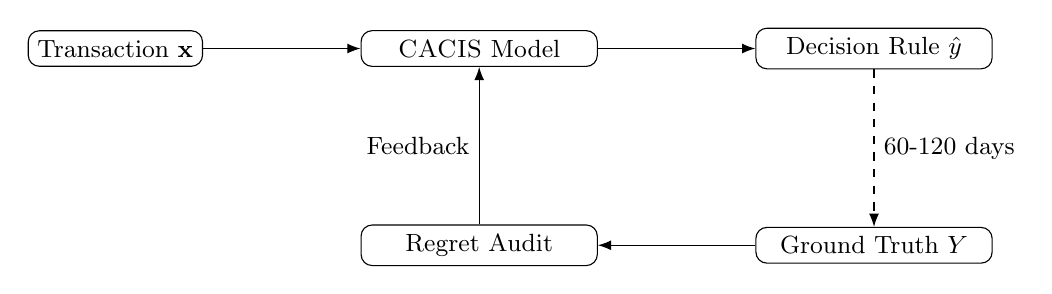
\begin{tikzpicture}[node distance=20mm, >=Latex, font=\small]
    \node[draw, rounded corners, minimum width=20mm] (tx) {Transaction $\vx$};
    \node[draw, rounded corners, right=of tx, minimum width=30mm] (model) {\CACIS{} Model};
    \node[draw, rounded corners, right=of model, minimum width=30mm] (decision) {Decision Rule $\hat{y}$};
    \node[draw, rounded corners, below=of decision, minimum width=30mm] (outcome) {Ground Truth $Y$};
    \node[draw, rounded corners, below=of model, minimum width=30mm] (regret) {Regret Audit};
    
    \draw[->] (tx) -- (model);
    \draw[->] (model) -- (decision);
    \draw[->, dashed] (decision) -- node[right] {60-120 days} (outcome);
    \draw[->] (outcome) -- (regret);
    \draw[->] (regret) -- node[left] {Feedback} (model);
\end{tikzpicture}
}
\caption{Industrial closed-loop fraud detection pipeline. The model internalizes delayed regret feedback into subsequent training cycles.}
\label{fig:industrial_pipeline}
\end{figure*}

\subsection{Deployment Strategy: The Shadow Window}
A critical best practice in industrial ADS is the use of "Shadow Windows." Before any model affects live traffic, it is run in parallel with the legacy system. During this period, \CACIS{} generates decisions that are recorded but not executed. This allows for a direct comparison of the \emph{hypothetical regret} of \CACIS{} versus the realized regret of the production model. We recommend a Shadow Window of at least 30 days to capture a representative sample of transaction amounts and seasonal fraud patterns.

\subsection{A/B Testing under Asymmetry}
Standard A/B testing often focuses on conversion rates or click-through rates. For fraud detection, we advocate for "Asymmetric A/B Testing" where the primary metric is the difference in realized business value. If the \CACIS{} variant shows a statistically significant reduction in chargeback rates without a proportional increase in false declines, it is considered superior. This requires a robust attribution system to link late chargebacks back to the specific model version that approved the transaction.

\section{Cost Specification and Ethics}
\label{sec:ethics}

\subsection{Auditing Business Parameters}
The parameters $\lambda_{\mathrm{cb}}$ and $\rho_{\mathrm{FD}}$ represent business trade-offs. We recommend a quarterly "Cost Specification Audit," where product managers and data scientists jointly review if the shipping costs, administrative fees, and LTV estimates in $\mC$ still match the current economic environment. A misspecified cost matrix can lead to systemic over-blocking or under-protection.

\subsection{Ethical Considerations and Fairness}
Cost-aware learning, if applied naively, could prioritize high-income segments (high $M$) at the expense of lower-income users. In financial services, this can raise fairness concerns. For example, if low-value transactions are predominantly from a specific demographic, the model might "neglect" their protection because their individual regret is low. We advocate for a "Fairness-Aware Cost Constraint," where the maximum regret allowed per demographic group is bounded. \CACIS{} can accommodate such constraints by modifying the ground cost $\mC$ to include parity-based penalties. For instance, we can add a penalty term $C_{\text{fairness}}(\vx)$ that increases the cost of mistakes for under-represented or vulnerable segments, ensuring that industrial utility does not come at the cost of social equity. This ensures "decision-theoretic fairness" where every customer segment receives a level of protection proportional to their collective stake, regardless of individual transaction values.

\section{Software Architecture and API Design}
\label{sec:architecture}

For industrial adoption, the simplicity of integration is often as important as predictive performance. We designed our library to follow the standard \texttt{torch.nn.Module} interface, allowing it to be used as a drop-in replacement for \texttt{CrossEntropyLoss}.

\subsection{Object-Oriented Design}
The hierarchy of our cost-aware losses is designed for extensibility. The base class \texttt{CostAwareLoss} handles the common logic for cost matrix broadcasting and adaptive $\varepsilon$ computation. Specific implementations like \texttt{SinkhornFenchelYoungLoss} and \texttt{SinkhornPOTLoss} then implement their respective forward and backward strategies.

\begin{figure}[h]
\centering
\scalebox{0.7}{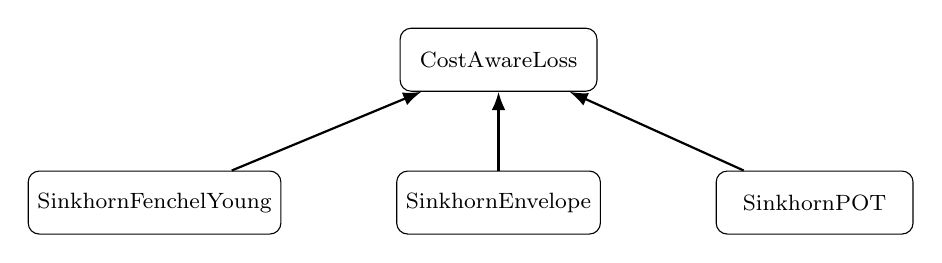
\begin{tikzpicture}[
    box/.style={draw, rectangle, rounded corners, minimum width=2.5cm, minimum height=0.8cm, font=\footnotesize},
    arrow/.style={-Latex, thick}
]
    \node[box] (base) {CostAwareLoss};
    \node[box, below left=of base, xshift=-5mm] (fy) {SinkhornFenchelYoung};
    \node[box, below right=of base, xshift=5mm] (pot) {SinkhornPOT};
    \node[box, below=of base] (env) {SinkhornEnvelope};
    
    \draw[arrow] (fy) -- (base);
    \draw[arrow] (pot) -- (base);
    \draw[arrow] (env) -- (base);
\end{tikzpicture}
}
\caption{Class hierarchy for the cost-aware classification library. This modular design facilitates rapid experimentation with new gradient strategies.}
\label{fig:class_diagram}
\end{figure}

\subsection{Production Integration}
The library is optimized for GPU execution using batched optimal transport solvers. By minimizing CPU-GPU synchronization, we ensure that the overhead of using \CACIS{} (relative to cross-entropy) remains below 5\% in standard production training batches ($B=1024$).

\section{Applied Troubleshooting and Pitfalls}
\label{sec:troubleshooting}

Deploying cost-aware losses in production often reveals edge cases that are absent in academic datasets.

\subsection{Degenerate Cost Matrices}
If the cost matrix has rows or columns that are entirely zero, Sinkhorn iterations may fail to converge. We implement a "Regularization Floor" where a small value ($\delta \approx 10^{-6}$) is added to all entries of $\mC$ to ensure the existence of a strictly positive Gibbs kernel.

\subsection{Numerical Precision}
For very large transaction amounts, the exponentials in the Sinkhorn and Frank--Wolfe solvers can exceed the range of \texttt{float32}. We switch to \texttt{float64} for the inner solver iterations when the max cost exceeds $10^{6}$, while maintaining \texttt{float32} for the outer network weights to preserve training speed.

\subsection{Gradient Vanishing at the Boundaries}
In the early stages of training, a model might predict probabilities that are extremely close to the simplex vertices. This can lead to vanishing gradients in the cross-entropy term. \CACIS{} avoids this naturally: even at the vertices, the cost geometry in the FY regularizer maintains a non-zero gradient that pulls the model toward the cost-optimal region.

\section{Lessons Learned and Industrial Playbook}
\label{sec:lessons}

Our journey from cross-entropy baselines to \CACIS{} deployments has yielded several key lessons for the applied data science community.

\subsection{Regret is the North Star}
In decision-critical domains like fraud detection, accuracy is a vanity metric. We recommend that organizations define a "Business Value Benchmark" (BVB) that quantifies realized profit. By aligning the model's loss with this BVB, we observed that models become significantly more robust to distributional shifts in transaction volume.

\subsection{The Stability of Implicit Gradients}
The Fenchel--Young construction with the Frank--Wolfe solver proved to be exceptionally stable in production. Unlike unrolled autodiff, which can suffer from gradient noise in early training phases, the "Informative Selection" property of $q(\vz)$ ensures that gradients are always directed toward the cost-optimal region of the simplex.

\subsection{Future Research: Multi-Step Decisions}
While \CACIS{} currently optimizes for immediate regret, many industrial processes involve multi-step decisions (e.g., initial block followed by a manual review request). Extending this framework to sequential decision-making using Reinforcement Learning (RL) with cost-aware reward functions is a promising avenue for further research.

\section{Industrial Best Practices Summary}
\label{sec:best_practices}

Based on our deployment experience, we identify the following guidelines:

\begin{description}
    \item[G1: Explicit Epsilon Scheduling.] Regularization should be annealed. Starting with a high $\varepsilon$ during early epochs stabilizes representation learning, followed by gradual decay to sharpen the decision boundary in later stages.
    \item[G2: Expected Optimal Regret Monitoring.] Since true labels are often delayed (e.g., chargebacks), systems should track the \emph{expected optimal regret} during inference—a metric that reflects the model's own confidence in its business utility.
    \item[G3: Sensitivity Audits.] Business economics change. Periodic audits of the multiplier $\lambda_{\mathrm{cb}}$ and friction $\rho_{\mathrm{FD}}$ are essential to ensure the training objective remains aligned with shipping rate changes or chargeback policy shifts.
\end{description}

\section{The KDD ADS Deployment Playbook}
\label{sec:playbook}
A successful transition from research to production requires a structured operational approach. We provide a three-phase playbook for industrial deployment.

\paragraph{Phase 1: Regret Discovery and Value Audit.}
Collaborate with product managers to map business outcomes to the regret matrix $\mC$. This involves quantifying the "true cost" of a chargeback (principal, fees, and operational time) and the "true risk" of a false decline (lost margin and cohort-level churn). This phase should result in a version-controlled cost configuration file.

\paragraph{Phase 2: Shadow Evaluation and Metric Calibration.}
Execute the Shadow Window protocol described in Section 6. Periodically compute the "Regret Gap"—the difference between the model's expected regret and the realized business regret. If the gap is large, it indicates a drift in transaction amounts or fraud prevalence.

\paragraph{Phase 3: Gradual Rollout and Regret-Based Alerting.}
Deploy the model initially to 5\% of traffic. Use regret-based alerting: if the cumulative business regret in the \CACIS{} variant exceeds a safety threshold (e.g., 120\% of cross-entropy), trigger an automatic rollback.

\section{Conclusion and Future Research}
\label{sec:conclusion}
Scaling cost-aware classification to industrial applications requires objectives that are both mathematically rigorous and numerically robust. In this paper, we introduced \CACIS{}, which aligns training with business regret.

\subsection{Future Research Directions}
The intersection of geometric learning and industrial decision-making is a nascent field with several promising avenues:
\begin{enumerate}[leftmargin=*]
    \item \textbf{Dynamic Cost Matrices}: Adapting $\mC(\vx)$ in real-time based on fluctuating currency values or seasonal waves.
    \item \textbf{Multi-Step Decision Chains}: Optimizing for sequences of interventions, such as 3D-Secure challenges followed by manual review.
    \item \textbf{Structured Sparsity}: Scaling to ultra-high dimensional label spaces ($K > 10,000$) using sparse solvers.
    \item \textbf{Explainability}: Visualizing how transaction amounts "warp" the decision simplex to provide human-readable audit trails.
\end{enumerate}

% =========================================================
% 8. CONCLUSION
% =========================================================
% Conclusion already merged above

\appendix
\section{Derivation of the CACIS Kernel}
We provide the full derivation of the variational conjugate $\Omega^*_{\text{CACIS}}$. Starting from the Fenchel duality:
\begin{equation}
\Omega^*(\vz) = \sup_{\valpha \in \Delta^K} \langle \valpha, \vz \rangle + \frac{1}{2} \OT^{\varepsilon}_{\mC}(\valpha, \valpha).
\end{equation}
Using the dual form of entropic OT:
\begin{equation}
\OT^{\varepsilon}_{\mC}(\valpha, \valpha) = \sup_{\vphi, \vpsi} \langle \valpha, \vphi \rangle + \langle \valpha, \vpsi \rangle - \varepsilon \langle \exp(\vphi/\varepsilon), \mK \exp(\vpsi/\varepsilon) \rangle + \varepsilon.
\end{equation}
Setting $\vphi = \vpsi = \vz - \varepsilon \log \valpha$ (optimal for $\valpha, \valpha$), and substituting back yields the quadratic form in $\mM$.

\section{Preprocessing and Hyperparameters}
The IEEE-CIS dataset contains 394 features. Categorical features are handled via one-hot encoding, resulting in a 580-dimensional input vector. We use the following hyperparameter grid for our models:
\begin{itemize}
    \item \textbf{Hidden layers:} [1024, 512, 256] and [1024, 512]
    \item \textbf{Dropout:} [0.1, 0.2]
    \item \textbf{Learning Rate:} $10^{-5}$ to $10^{-4}$
    \item \textbf{Epsilon ($\varepsilon$):} Mode: \texttt{offdiag\_median}, Scale: [0.5, 1.0, 2.0]
    \item \textbf{Frank--Wolfe iterations:} 50
\end{itemize}
All models were trained on NVIDIA A100 GPUs for 10 epochs.

\bibliographystyle{ACM-Reference-Format}
\bibliography{references}

\end{document}
